%%
%% This is file `sample-sigplan.tex',
%% generated with the docstrip utility.
%%
%% The original source files were:
%%
%% samples.dtx  (with options: `sigplan')
%% 
%% IMPORTANT NOTICE:
%% 
%% For the copyright see the source file.
%% 
%% Any modified versions of this file must be renamed
%% with new filenames distinct from sample-sigplan.tex.
%% 
%% For distribution of the original source see the terms
%% for copying and modification in the file samples.dtx.
%% 
%% This generated file may be distributed as long as the
%% original source files, as listed above, are part of the
%% same distribution. (The sources need not necessarily be
%% in the same archive or directory.)
%%
%% Commands for TeXCount
%TC:macro \cite [option:text,text]
%TC:macro \citep [option:text,text]
%TC:macro \citet [option:text,text]
%TC:envir table 0 1
%TC:envir table* 0 1
%TC:envir tabular [ignore] word
%TC:envir displaymath 0 word
%TC:envir math 0 word
%TC:envir comment 0 0
%%
%%
%% The first command in your LaTeX source must be the \documentclass command.
\documentclass[sigplan,screen]{acmart}
%% NOTE that a single column version is required for 
%% submission and peer review. This can be done by changing
%% the \doucmentclass[...]{acmart} in this template to 
%% \documentclass[manuscript,screen,review]{acmart}
%% 
%% To ensure 100% compatibility, please check the white list of
%% approved LaTeX packages to be used with the Master Article Template at
%% https://www.acm.org/publications/taps/whitelist-of-latex-packages 
%% before creating your document. The white list page provides 
%% information on how to submit additional LaTeX packages for 
%% review and adoption.
%% Fonts used in the template cannot be substituted; margin 
%% adjustments are not allowed.
%%
%% \BibTeX command to typeset BibTeX logo in the docs
\AtBeginDocument{%
  \providecommand\BibTeX{{%
    \normalfont B\kern-0.5em{\scshape i\kern-0.25em b}\kern-0.8em\TeX}}}

%% Rights management information.  This information is sent to you
%% when you complete the rights form.  These commands have SAMPLE
%% values in them; it is your responsibility as an author to replace
%% the commands and values with those provided to you when you
%% complete the rights form.
\setcopyright{acmcopyright}
\copyrightyear{2018}
\acmYear{2018}
\acmDOI{XXXXXXX.XXXXXXX}

%% These commands are for a PROCEEDINGS abstract or paper.
\acmConference[Conference acronym 'XX]{Make sure to enter the correct
  conference title from your rights confirmation emai}{June 03--05,
  2018}{Woodstock, NY}
%
%  Uncomment \acmBooktitle if th title of the proceedings is different
%  from ``Proceedings of ...''!
%
%\acmBooktitle{Woodstock '18: ACM Symposium on Neural Gaze Detection,
%  June 03--05, 2018, Woodstock, NY} 
\acmPrice{15.00}
\acmISBN{978-1-4503-XXXX-X/18/06}


%%
%% Submission ID.
%% Use this when submitting an article to a sponsored event. You'll
%% receive a unique submission ID from the organizers
%% of the event, and this ID should be used as the parameter to this command.
%%\acmSubmissionID{123-A56-BU3}

%%
%% For managing citations, it is recommended to use bibliography
%% files in BibTeX format.
%%
%% You can then either use BibTeX with the ACM-Reference-Format style,
%% or BibLaTeX with the acmnumeric or acmauthoryear sytles, that include
%% support for advanced citation of software artefact from the
%% biblatex-software package, also separately available on CTAN.
%%
%% Look at the sample-*-biblatex.tex files for templates showcasing
%% the biblatex styles.
%%

%%
%% The majority of ACM publications use numbered citations and
%% references.  The command \citestyle{authoryear} switches to the
%% "author year" style.
%%
%% If you are preparing content for an event
%% sponsored by ACM SIGGRAPH, you must use the "author year" style of
%% citations and references.
%% Uncommenting
%% the next command will enable that style.
%%\citestyle{acmauthoryear}

%%
%% end of the preamble, start of the body of the document source.
\begin{document}

%%
%% The "title" command has an optional parameter,
%% allowing the author to define a "short title" to be used in page headers.
\title{The Name of the Title is Hope}

%%
%% The "author" command and its associated commands are used to define
%% the authors and their affiliations.
%% Of note is the shared affiliation of the first two authors, and the
%% "authornote" and "authornotemark" commands
%% used to denote shared contribution to the research.

%---Copy paste this 
\author{Name Surname}
\affiliation{%
  \institution{Saarland University}
  \country{Germany}
  \postcode{66123}}
\email{uni-email@saarland.de}


%%
%% The abstract is a short summary of the work to be presented in the article.
\begin{abstract}
  Here goes your abstract in max 250 - 300 words. As only one paragraph, summarizing the interest of your work. Remember the main points : 
\begin{itemize}
    \item 1st paragraph: explain why the issue is really important Here is the answer to the question "what is the context and why does this matter", to the society or a group of people.
    \item 2nd paragraph : explain your specific question that although it matters a lot, we don’t have much coverage for it. Although it matters to the community for the reasons above, this is the current state of the situation : we found something that is missing or is not adapted and there's not much related work about this
    \item 3rd paragraph : explain on what your research design focuses, what data it relies on, and what methods it uses, as well as what you have learned about the question and what are the implications. We saw why it matters, we know the situation and identified what is missing, so here is our solution to fill in this gap in a concise phrase and one that gives the main points of the solution.
\end{itemize}
This is an example of how to include a hyperlink \href{https://www.fabriziogilardi.org/resources/papers/good-abstracts.pdf}{Abstract method example by Fabrizio Gilardi} 

NOTE : Pay attention to the commented paragraph below in the code.
\end{abstract}

%%
%% The code below is generated by the tool at http://dl.acm.org/ccs.cfm.
%% Please copy and paste the code instead of the example below. Choose Human-centered computing -> HCI -> Interaction devices -> .... (the best choice based on your project)
%%
\begin{CCSXML}
<ccs2012>
   <concept>
       <concept_id>10003120.10003121.10003125</concept_id>
       <concept_desc>Human-centered computing~Interaction devices</concept_desc>
       <concept_significance>500</concept_significance>
       </concept>
 </ccs2012>
\end{CCSXML}

\ccsdesc[500]{Human-centered computing~Interaction devices}

%%
%% Keywords. The author(s) should pick words that accurately describe
%% the work being presented. Separate the keywords with commas.
\keywords{ 3 - 5 keywords}

%% A "teaser" image appears between the author and affiliation
%% information and the body of the document, and typically spans the
%% page.
\begin{teaserfigure}
  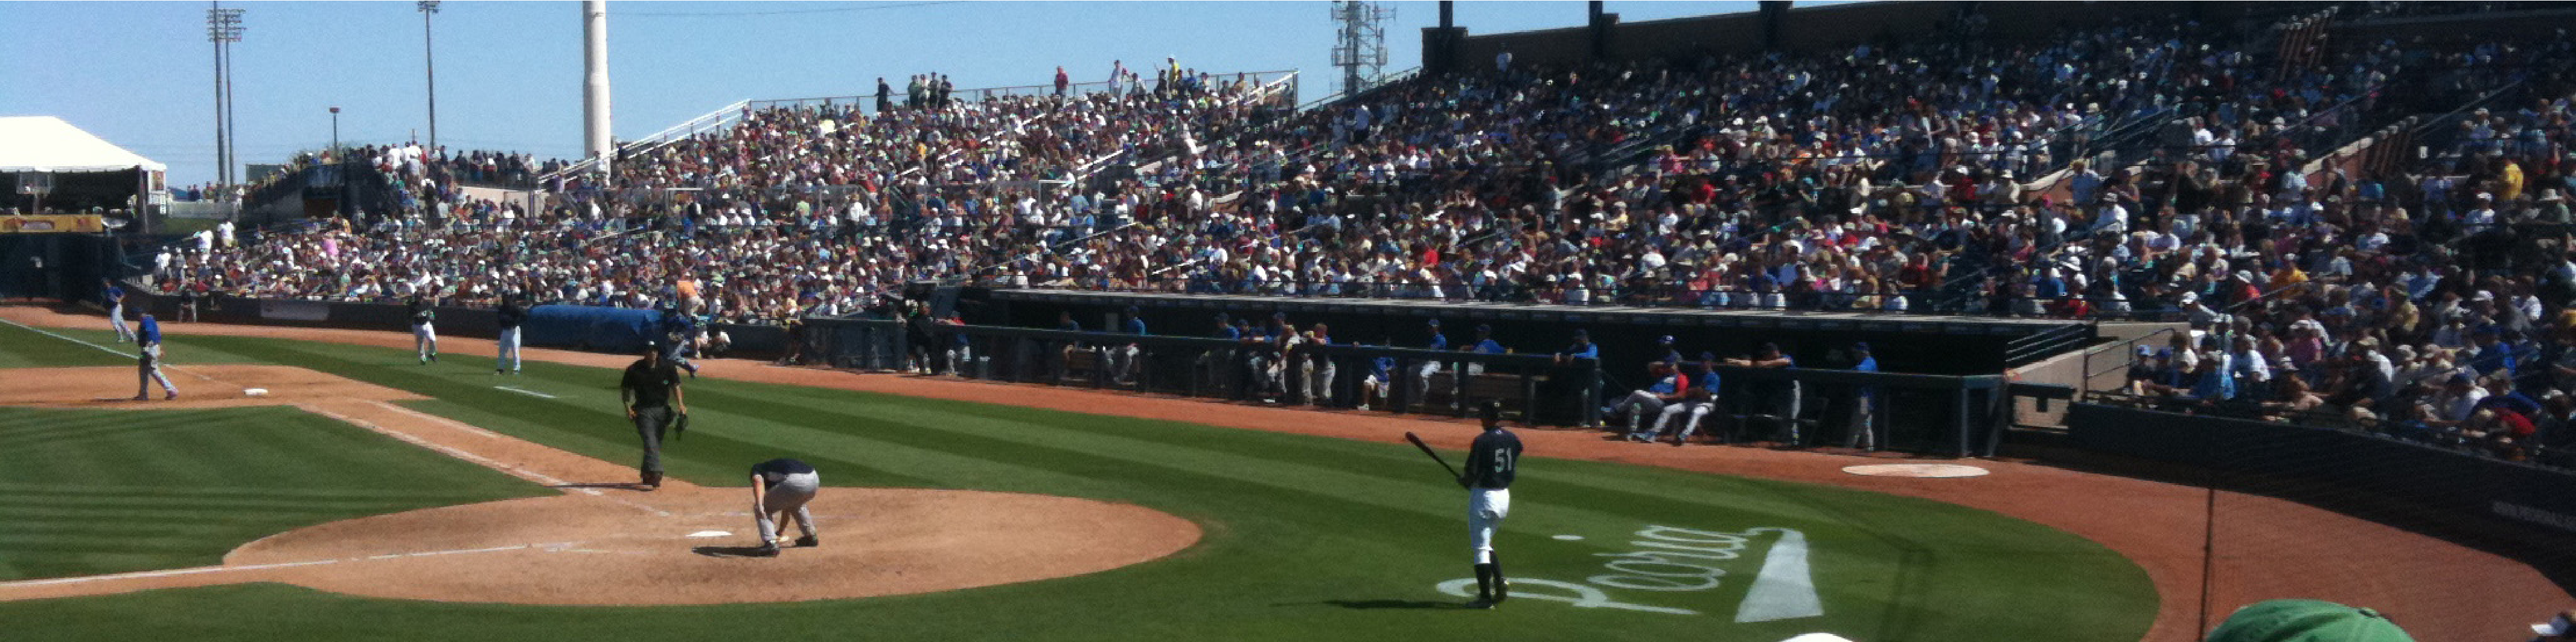
\includegraphics[width=\textwidth]{sampleteaser}
  \caption{Seattle Mariners at Spring Training, 2010.}
  \Description{Enjoying the baseball game from the third-base
  seats. Ichiro Suzuki preparing to bat.}
  \label{fig:teaser}
\end{teaserfigure}

%%
%% This command processes the author and affiliation and title
%% information and builds the first part of the formatted document.
\maketitle

\section{Introduction}
Here goes the ameliorated version of the introduction you wrote for the previous milestone, based on the feedback and the evolution of your thoughts. This section can include some references of the domain if needed, however they remain general.
Remember the introduction follows the same plan as the abstract and elaborates each of the summarized parts. 
\begin{itemize}
    \item Motivation - Setting the stage and suggesting why the coming problem should be relevant
    \item Problem - Phrase the problem precisely that you are about to tackle. These problems/challenges need to have a clear and strong mapping to your contribution. Do NOT name any problems that your project/contribution does not solve.
    \item Solution - Now I understand the problem and care for it because of the motivation. Now tell me how you think you solved it
    \item Method - Ok interesting so now tell me a little bit about how you did that 
\end{itemize}

Remember the speech remains mostly impersonal, using pronouns as "we" or expressions like "in this work", "this concept/project presents" etc. You're supposed to be concise and factual, every phrase is supposed to give the lecturer a piece on valuable information.
\section{Related Work}
In this section you should reformulate your previous related work or complete it with new references. You can keep it split in blocks if you have difficulities but the aim is to create links between your references and whee what is common, what are their contributions, what is missing and compare them. Here is Marie's poster \cite{muehlhaus2022feather} associated with the video cited earlier. 
\section{XXXXX}
This section includes the techincal/social parts and everything that leads to the final design of your project. It also includes the use cases that are presented as applications. You can create a different subsection for each different context of applications, the title of the subsection being the most important factor that changes your context ( e.g. for the plant watering system : "Traveler Lifestyle", "Limited mobility", "Mental well-being" etc.)
\section{Evaluation and Results}
You won't have an evaluation section as developed as Marie. However please describe the results you got : for example ask your parents what they think about this, or ask your siblings to use the prototype and tell us what happened, what did they said. Do not provide names or any personal details, use only their profile like their age and job / hobby / lifestyle/etc if relevant. 
You should create subsections that evaluate different aspects of your project. For example (not all mandatory) : 
\subsection{Design}
... description of what your users said and a final phrase with your analysis and conclusions
\subsection{Interaction}
... description of what your users said and a final phrase with your analysis and conclusions
\subsection{Ergonomics}
... description of what your users said and a final phrase with your analysis and conclusions

You can include tables by zooming and screenshot-ting your screen ( or you can deal with real LateX tables, good luck ) using the same code as for this image.

\begin{figure}[h]
    \centering
    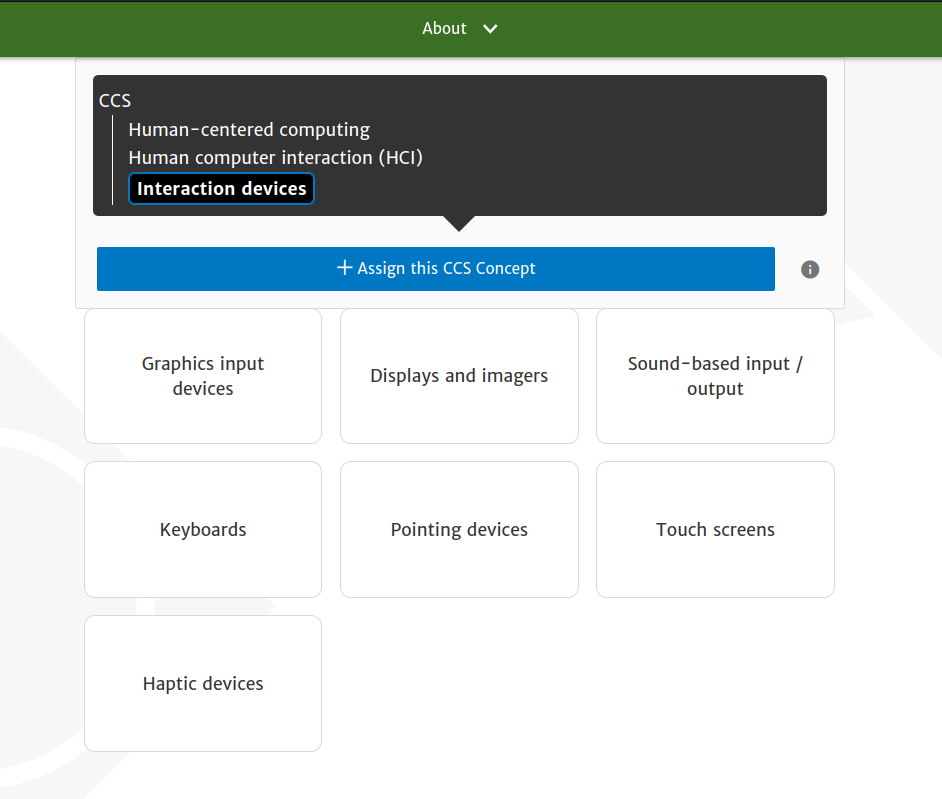
\includegraphics[width=1\columnwidth]{Figures/example.png}
    \caption{Sample image guiding for the choice of concepts on acm website}
    \label{fig:sample}
\end{figure}



\section{Conclusion}
The conclusion should be short not going further than 2/3 of a column.




%%
%% The acknowledgments section is defined using the "acks" environment
%% (and NOT an unnumbered section). This ensures the proper
%% identification of the section in the article metadata, and the
%% consistent spelling of the heading.
\begin{acks}
To Robert, for the bagels and explaining CMYK and color spaces.
\end{acks}

%%
%% The next two lines define the bibliography style to be used, and
%% the bibliography file.
\bibliographystyle{ACM-Reference-Format}
\bibliography{sample-base}

\end{document}
\endinput
%%
%% End of file .
